\begin{frame}
\frametitle{The Barrel and the Wheel}

\blt\ The idea of measuring \sone\ and/or \stwo\ using a WLS was proposed by DN many years ago. He suggested to possibilities. A barrel and a wheel. The barrel would run along the field cage, while the wheel could be place in the anode. In both cases, the detector would be a WLS plastic coated with another WLS, such as TPB or TPH. The role o the TPB (TPH) would be to shift impinging VUV light to blue light, that would then be capture by the barrel or the wheel and propagate by total internal reflection (TIR) to readout. 

\blt\ The problem with this implementation is that TPB (TPH) has the same refraction index that poly ($\sim 1.6$), and thus the light would end up propagating in the interface between TPB and xenon (which has much lower refraction index, $\sim 1$). But, since such a surface is very inhomogeneous, transmittance vanished quickly.
\end{frame}

\begin{frame}
\frametitle{Crying WOLF}

\blt\ A solution to this problem (JJGC, JMV, FM) is using Wavelength sifter OpticaL Fibres (WOLFs), which include one (or two) claddings ($n \sim 1.49$) which prevent light from reaching the TPB surface. Transmission is then restored. 

\blt\ Further advantages of WOLFs w.r.t. other solutions (such as the ARAPUCA designs, for DUNE) are robustness, availability (they are produce by two large manufacturers, Kuraray and St. Gobain) and cost.  

\blt\ In this way, both the Barrel and the Wheel (or rather the Wall) detectors can be resurrected. We call them BFD (Barrel Fibre detector) and AFD (Anode Fibre detector).  

\end{frame}

\begin{frame}
\frametitle{Principle of operation}
\begin{columns}
\column{0.45\textwidth}

\blt\ The basic component is a wavelength-shifting (WLS) optical fibre coated with TPB or another suitable VUV$\rightarrow$Blue WLS. The fibre itself is made of a polystyrene core ($n=1.6$) and an acrylic (double) cladding ($n=1.49$).

\blt VUV impinging upon the fibre is shifted to blue and enters the fibre where is eventually shifted to green and propagates by total internal reflection.
\column{0.45\textwidth}
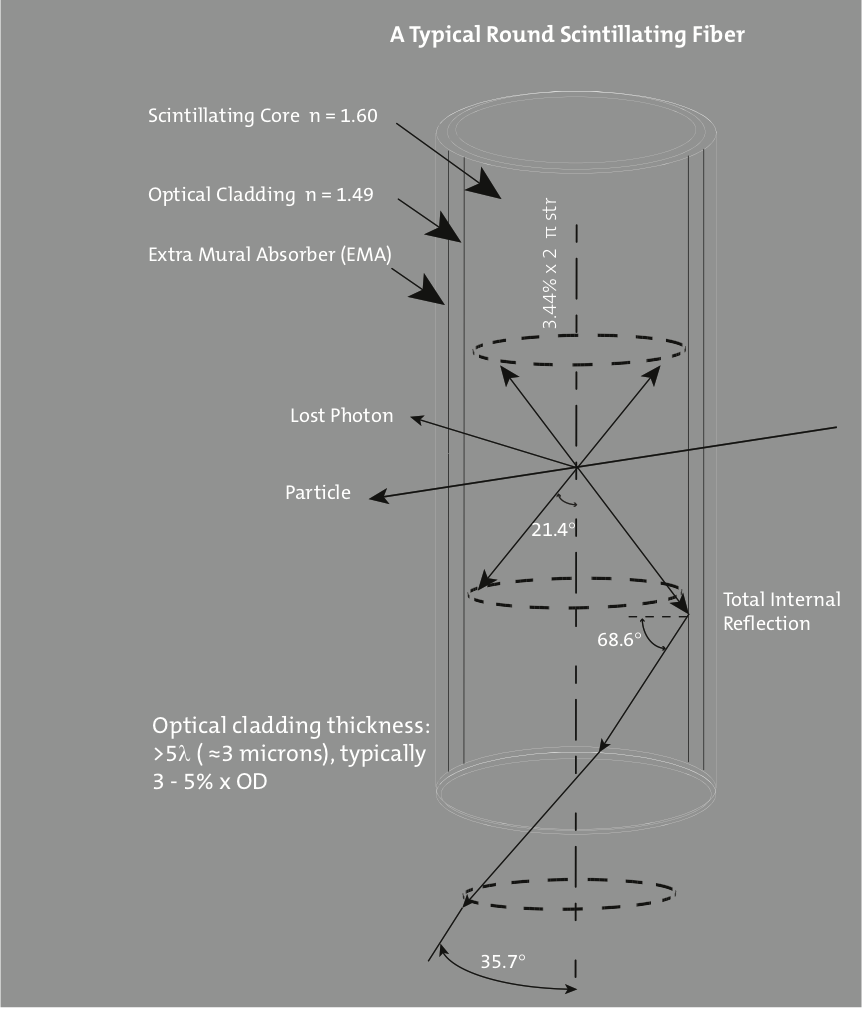
\includegraphics[scale=0.6]{img/fibers_tirf.png}

\end{columns}

\end{frame}


%\begin{frame}
%\frametitle{What is a field?}
%
%\begin{tcolorbox}[colback=white,arc=0pt,outer arc=0pt,colframe=black,boxrule=0.6pt]
%  \begin{center}
%    A field is a {\em device} that operates over a position in spacetime, $x^{\mu}$~ to produce an object representing the amplitude of something at that point in spacetime, $\phi(x^{\mu})$. The amplitude can be a {\em scalar}, a {\em vector}, a {\em complex number}, a {\em spinor} or a {\em tensor}. 
%
%  \end{center}
%\end{tcolorbox}
%
%\blt\ The concept of a field as an unseen entity which pervades space and time, connects with the concept of {\em ether}. 
%
%\blt\ Faraday grasped intuitively the idea of an electric or magnetic field that permeates all space and time. Maxwell codified Faraday?s idea and the electromagnetic field, together with all the paraphernalia of field theory, was born. 
%
%\blt\ In classical physics we understand that gravity is a field, electromagnetism is a field, and each can be described by a set of equations which governs their behavior. The field can oscillate in space and time and thus wave-like excitations of the field can be found (electromagnetic waves are well-known, and gravity waves have recently been observed). 
%
%\blt\ The advent of quantum mechanics removed the distinction between what had been thought of as wave-like objects and particle-like objects. Therefore even matter itself is an excitation of a quantum field and quantum fields become the fundamental objects which describe reality.
%
%
%\end{frame}

